\documentclass[11pt,a4paper,onecolumn]{IEEEtran}
\usepackage[margin=3cm]{geometry}
\usepackage[english]{babel}
\usepackage{graphicx}
\usepackage{lipsum}
\usepackage{listings}[language=Javascript]
% Path relative to the .tex file containing the \includegraphics command
\graphicspath{ {./images/} }

\title{Promsie\\
{\footnotesize RWTH Aachen University}}

\author{
  \IEEEauthorblockN{1\textsuperscript{st} Papop Lekhapanyaporn}
  \and
  \IEEEauthorblockN{2\textsuperscript{nd} Tobias Piatek}
  \and
  \IEEEauthorblockN{3\textsuperscript{rd} Tobias Waerder}
  }



\begin{document}
\maketitle

\begin{abstract}
  In Javascript there are two ways to handle asynchronous code. The first way is to use callbacks. The second way is to use promises. This paper will explain the concept of promises and how to use them. The paper will also compare the two ways to handle asynchronous code.
\end{abstract}

\section{eventloop}
In Javascript, a single threaded programming language, It is possible to handle thousands of operation symaltaniously by 
using eventloop. Eventloop is created to fix the single threaded problem that program can only run one function at a time. 
In practice, the program will be unusable without event loop. 
\begin{figure}[h]
  \centering
  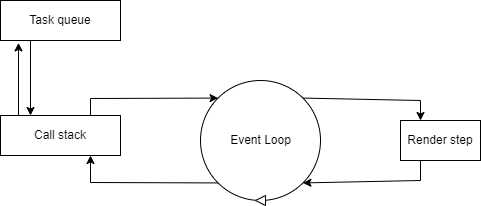
\includegraphics[scale=0.5]{eventloop}
  \caption{eventloop}
  \label{fig:eventloop}
\end{figure}

in figure \ref{fig:eventloop} the eventloop will constantly check the task queue. 
If there is a task in the task queue, the first task in the queue will be removed and put into the call stack.
The eventloop will then take a detour to the call stack and execute the task that was in the callstack.
After a certain amount of time has passed the event loop will then go through the render step which contain styles generation,
layout positioning , and pixel data generation that will be displayed on the browser.
\section{callbacks}

\section{Promises}
Promise is a object use to represent a task that will eventually be either be fullfilled or rejected. 
if the Task is fullfilled, then the promise will be resolved. If the task is rejected, then the promise will be rejected.
\begin{lstlisting}
  const promise = new Promise((resolve,reject)=>{
    setTimeout(()=>{
      resolve('done');
    },1000);
  });
\end{lstlisting}
\subsection{Callback Handling} 
Promise will eventually either be fullfilled or rejected. 

\subsubsection{then()}
then can be use to handle the fullfilled promise.
\begin{lstlisting}
  promise.then()
\end{lstlisting}

\subsubsection{catch()}
catch can be use to handle the rejected promise.
\begin{lstlisting}
  promise.catch()
\end{lstlisting}

\subsection{Chaining}
Promise can be chained together to handle multiple asynchronous funtion. often use when fetching data from HTTP server and convert to json.
\begin{lstlisting}
  promise.then().then().catch()
\end{lstlisting}
\subsection{Catching Errors}
\subsection{fetch API}
fetch API is a promise based API that can be use to make HTTP request. 
\begin{lstlisting}
  const res = fetch('...');
\end{lstlisting}

\section{Asynchronous methods}
\subsection{async}
\subsection{await}

\section{Conclusion}
\begin{thebibliography}{9}
  \bibitem{article} Author,Title \emph{Bookname}, Band and publication number,Page,Year.
  \bibitem{conferences} Author, TItle \emph{Conference Name}, Page, Year
  \bibitem{book} Author, \emph{Title}, Publisher, Year
\end{thebibliography}
\end{document}
references not counted toward the page limit (12 pages)
tips
- no singular pronouns (I)
-keywords write as cursive
- limited the use of footnotes
-examples
- every concept should have a example
- if possible use only one example
- use a example that is easy to understand

